\section {Introduction\\}
Traditionally, the web server is a classical example of the request/response 
model, where the clients can retrieve the resource from the server but the 
server cannot push the data to the client directly. 

However, with the increasing popularity of Ajax\cite{Ajax} technologies, there 
are many scenarios where servers would like to actively notify the clients the 
latest updates. For example, the new messages in chat room, latest tweets in 
twitter, etc.

To overcome the limitation of request/response model, many approaches has been 
proposed to build more responsive sites. For example:

\begin{itemize}
\item Client Pull: the client sends update requests periodically to pull the
updates from server. This method is very easy to implement because 
it is stateless and the web server doesn't need to put much effort to modify 
its existing architecture. However, client pull will generate lots of http requests.
The work flow of client pull is illustrated in Figure \ref{fig:client_pull}.

\item Plugins: since the HTTP itself doesn't provide any mechanism for server 
push, plugins, such as the Flash, Silverlight, Javelet, etc, can be used as an 
extension of the HTTP by providing more flexible client/server communication 
mechanisms. However plugins is non-standard and requires users' extra effort to 
install and configure them.
\end{itemize}

Given those drawbacks, we consider another solution: long polling
\cite{LongPolling}. The work flow of long polling can be described in Figure
\ref{fig:long_polling}. When a client ``asks for"(polls) an update by sending 
an HTTP request to the server, if no information is yet available, the 
server will not terminate the connection immediately; Instead, the server 
will keep the connection open for a period of time until (1) the information 
become available (2) after a suitable timeout($50$ seconds is a common choice
in many commercial websites).

The benefit to long-polling is that there is less back-and-forth between the 
client and server. The server is in control of the timing, so updates to the
browser can normally be made within milliseconds. This makes it ideal for 
some highly interactive web applications.

\begin{figure}[htb!]
\centering
    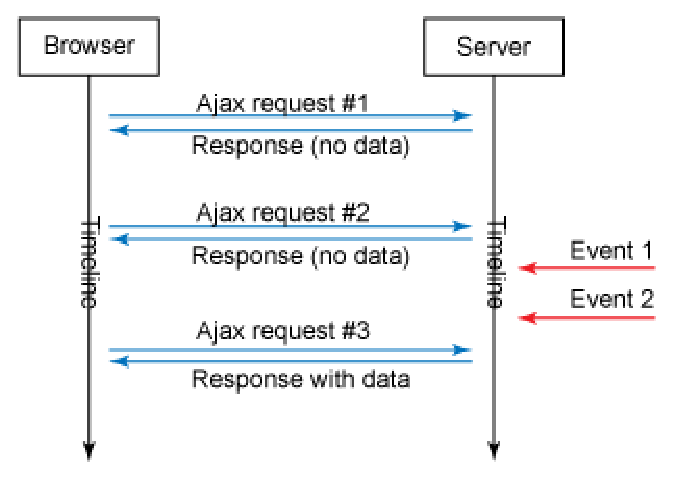
\includegraphics[scale=0.85]{figures/client_pull.eps}
    \caption{Client Pull Work Flow}
    \label{fig:client_pull}
\end{figure}

\begin{figure}[htb!]
    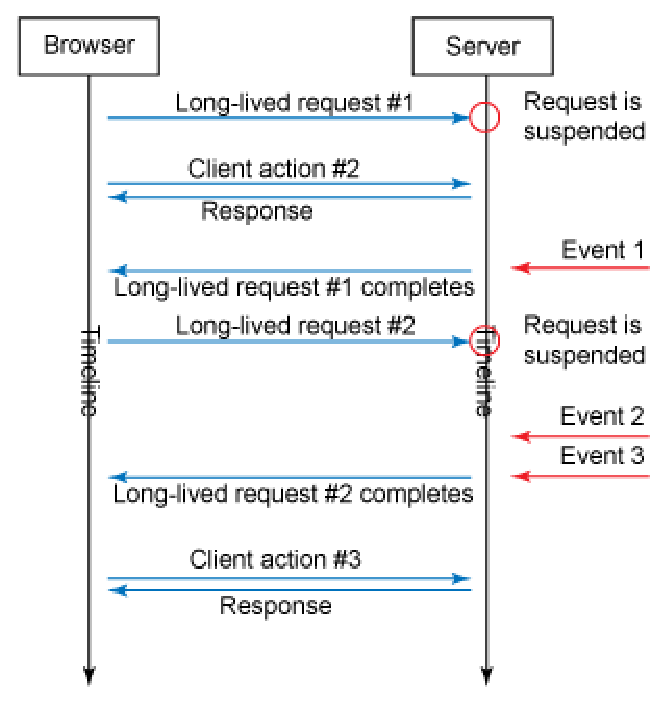
\includegraphics[scale=0.80]{figures/long_polling.eps}
    \caption{Long Polling Work Flow}
    \label{fig:long_polling}
\end{figure}

The down-side of long polling is that the server may have to deal with large
amount of active connections between the clients and the servers. For example,
suppose a website has one million registered users, of which 10\% are online at any 
time. This means that the server must able to hold at least 100,000 concurrent 
connections if it chooses to employ long polling.

To address these problems, we present the event-driven, scalable
long polling server \textbf{PushUp} to provide dedicated long polling services for 
different web applications with less resource cost.

As illustrated in Figure \ref{fig:sim_pushup}, the PushUp server, designed
as a dedicated long polling server, introduces an intermediary between
the clients and web servers. Inside the PushUp server there is a specialized 
event-driven message queue that:
\begin {itemize}
    \item[1] Keeps the active connections with low overhead.
    \item[2] Provides a familiar interface for clients to listen to the latest 
             updates and the web servers to notify the newest changes.
\end {itemize}


\begin{figure}[htb!]
\centering
    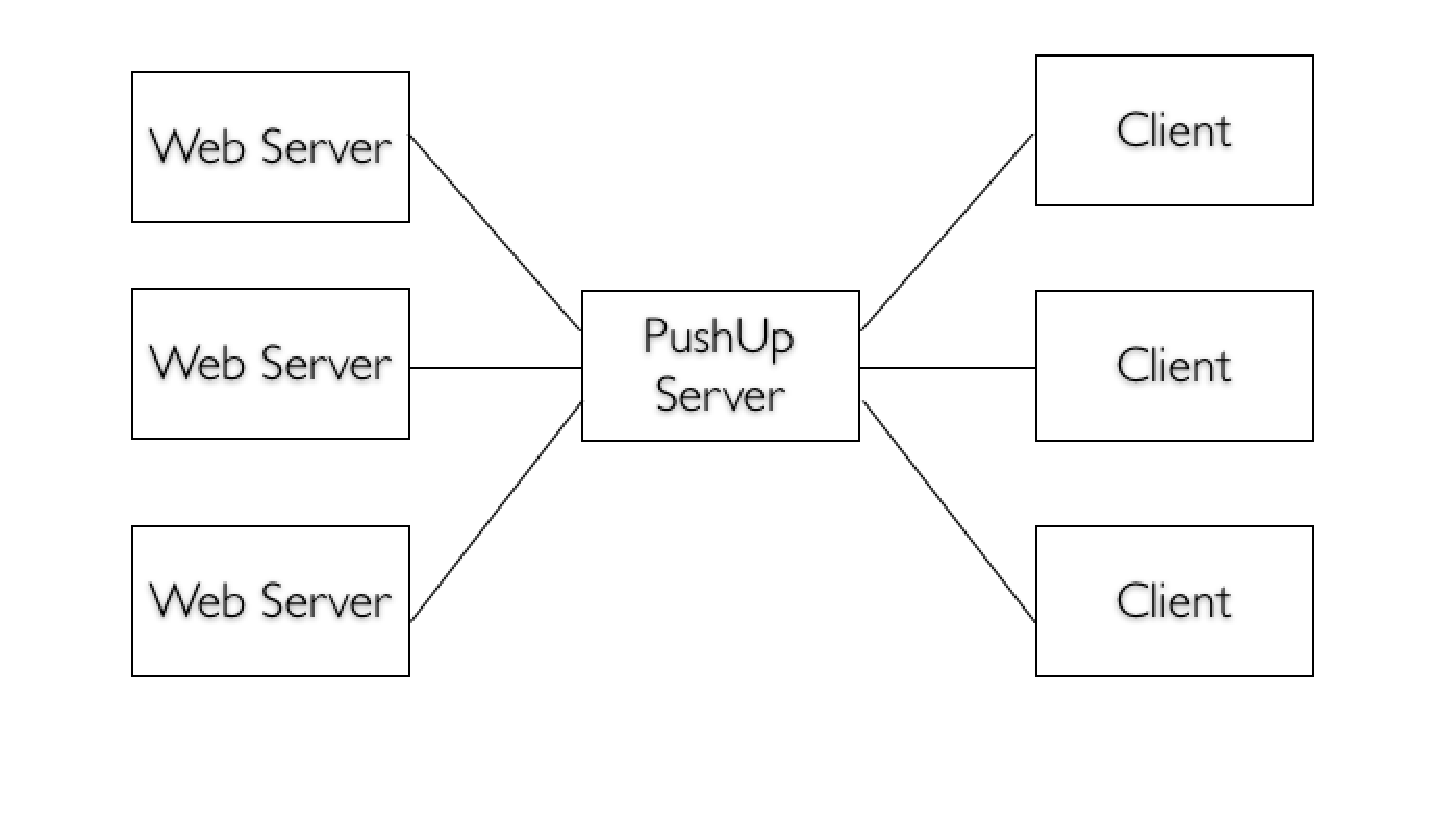
\includegraphics[scale=0.40]{figures/sim_pushup.eps}
    \caption{Simplified Architecture of the PushUp}
    \label{fig:sim_pushup}
\end{figure}
